\newpage
\section{Proiecția ortografică}

Proiecția ortografica (sau proiecția ortogonala) este o modalitate de a reprezenta un model tridimensional  
într-un spațiu bidimensional. Este o forma de proiecție paralela, în care toate liniile de proiecție sunt ortogonale 
cu planul de proiecție.\newline

Termenul ortografic este uneori rezervat în mod specific pentru reprezentări ale obiectelor în care axele principale 
sau planurile obiectului sunt de asemenea paralele cu planul de proiecție, dar acestea sunt mai bine cunoscute 
ca proiecții multiview. Mai mult, atunci când planurile sau axele principale ale unui obiect într-o proiecție 
ortografică nu sunt paralele cu planul de proiecție, dar sunt înclinate mai degrabă pentru a descoperi mai 
multe laturi ale obiectului, proiecția se numește o proiecție axonometrică. Subtipurile de proiecție multiview 
includ planuri, elevații și secțiuni. Subtipurile de proiecții axonometrice includ proiecții izometrice, dimetrice și trimetrice. \newline

\begin{figure}[H]
  \begin{center}
      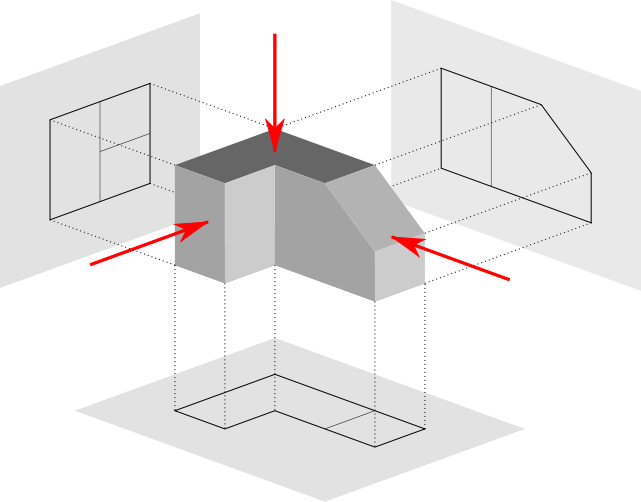
\includegraphics[scale=0.5]{imagini/proiectie/ortografica.png}
      \caption{Proiecția ortografică a unui corp}
      \label{fig:tabs}
  \end{center}    
\end{figure}

O proiecte ortografica simpla, pe planul \(z=0\) poate fi definita de urmatoarea matrice:

\[
P=
  \begin{bmatrix}
    1 & 0 & 0 \\
    0 & 1 & 0 \\
    0 & 0 & 0 
  \end{bmatrix}
\]

Pentru fiecare punct \(v=(v_x,v_y,v_z)\), punctul transformat ar fi:

\[
P_v=
  \begin{bmatrix}
    1 & 0 & 0 \\
    0 & 1 & 0 \\
    0 & 0 & 0 
  \end{bmatrix}
  \begin{bmatrix}
    v_x  \\
    v_y  \\
    v_z  
  \end{bmatrix}
  =
  \begin{bmatrix}
    v_x  \\
    v_y  \\
    0  
  \end{bmatrix}
\]

\subsection{Aplicare}

Acest concept a fost aplicat pentru reprezentarea elementelor care formeaza intregrul model 3D. 
Setul de date nu contine dimensiunile exacte ale elementelor ci doar punctele de legare cu late elemente si centrul de greutate.
Prin calcularea punctelor simetrice ale punctelor de legare la centrul de greutate și prin incadrarea unui dreptunghi in jurul lor
obtinem forma care v-a reprezenta elementul in sine.\newline 

Aplicația conține trei moduri de afișare a modelului, fiecare perspectivă folosind coordonatele \((x,y,z)\) din setul de date 
eliminand una din ele pentru reprezentarea in 2D:
\begin{itemize}
\item Perspectva de deasupra, folosind \((x,y)\)     
\item Perspectva laterală, folosind \((x,z)\)
\item Perspectva frontala, folsind \((y,z)\)
\end{itemize}